\section{Introduction} \label{sec:intro}
%%%%%%%%%%%%%%%%%%%%%%%%%%%%%%%%%%%%%%%%%%%%

Random regular graphs,
where each vertex has the same degree $d$,
are among the most well-known examples of {\it expanders}:
graphs with high connectivity and which exhibit rapid mixing.
Expanders are of particular interest in computer science, 
from sampling and complexity theory to design of error-correcting codes.
For an extensive review of their applications, see \cite*{hoory2006}.
What makes random regular graphs particularly interesting expanders 
is the fact that they exhibit all three existing
types of expansion properties: edge, vertex, and spectral. 

The study of regular random graphs took off with the work of
\citet*{bender1974}, \citet*{bender1978},
\citet*{bollobas1980},
and slightly later \citet*{mckay1984} and \citet*{wormald1981}. 
Most often, their expanding properties are described 
in terms of the existence of the \emph{spectral gap}, which we define below. 

Let $A$ be the adjacency matrix of a simple graph,
where $A_{ij} = 1$ if $i$ and $j$ are connected and zero otherwise.
Denote
$\sigma(A) = \{\lambda_1 \geq \lambda_2 \geq \ldots \}$
as its spectrum. 
For a random $d$-regular graph, $\lambda_1 = \max_{i} |\lambda_i| = d$, 
but the second largest eigenvalue
$\eta = \max (|\lambda_2|, |\lambda_{n}| )$ 
is asymptoticly almost surely 
of much smaller order, leading to a spectral gap.
Note that we will always use $\eta$ to be the second largest 
eigenvalue of the adjacency matrix $A$.
For a list of important symbols see Appendix~\ref{sec:list_of_symbols}.

Spectral expansion properties of a graph are, strictly speaking,
defined with respect to the smallest nonzero eigenvalue of the normalized Laplacian,
$\mathcal{L} = I - D^{-1/2} A D^{-1/2}$, 
where $I$ is the identity and $D$ is the diagonal matrix of vertex degrees.
In the case of a $d$-regular graph, $\sigma(\mathcal{L})$ is a scaled
and shifted version of $\sigma(A)$.
Thus, a spectral gap for $A$ translates directly into one for $\mathcal{L}$.

The study of the second largest eigenvalue in regular graphs 
had a first breakthrough in the Alon-Boppana bound 
\citet*{alon1986},
which states that the second largest eigenvalue satisfies
\[
 \eta \geq 2 \sqrt{d-1} - \frac{c_d}{\log n} .
\]
Graphs for which the Alon-Boppana bound is attained are called {\it Ramanujan}.
\citet*{friedman2003a} proved the conjecture of \citet*{alon1986} that
almost all $d$-regular graphs have $\eta \leq 2 \sqrt{d-1} + \epsilon$
for any $\epsilon > 0$
with high probability as the number of vertices goes to infinity. This result was simultaneous simplified and deepened in \citet*{friedman2014}. 
More recently, \citet*{bordenave2015} gave a different proof that
$\eta \leq 2 \sqrt{d-1}+\epsilon_n$ 
for a sequence $\epsilon_n \rightarrow 0$ as $n$, 
the number of vertices, tends to infinity; the new proof is based on the non-backtracking operator and the Ihara-Bass identity.  

\subsection{Bipartite biregular model}

In this paper we prove the analog of Friedman and Bordenave's result 
for bipartite, biregular random graphs. 
These are graphs for which the vertex set partitions into two independent
sets $V_1$ and $V_2$, such that all edges occur between the sets.
In addition, all vertices in set $V_i$ have the same degree $d_i$.
See Figure~\ref{fig:bipartite_schematic} for a schematic of such a graph.
Along the way, we also bound the smallest positive eigenvalue and
the rank of the adjacency matrix.

Let $\mathcal{G}(n,m,d_1,d_2)$ be the uniform distribution of
simple, bipartite, biregular random graphs. 
Any $G \sim \mathcal{G}(n,m,d_1,d_2)$ 
is sampled uniformly from the set of simple bipartite graphs 
with vertex set $V=V_1 \bigcup V_2$, 
with $|V_1|=n$, $|V_2|=m$ 
and where every vertex in $V_i$ has degree $d_i$. 
Note that we must have $n d_1 = m d_2 = |E|$.
Without any loss of generality, we will assume $n \leq m$
and thus $d_1 \geq d_2$
when necessary.
Sometimes we will write that $G$ is a $(d_1, d_2)$-regular graph, 
when we want to explicitly state the degrees.
Let $X$ be the $n \times m$ matrix with entries $X_{ij}=1$ 
if and only if there is an edge between vertices 
$i \in V_1$ and $j \in V_2$. 
Using the block form of the adjacency matrix
\begin{equation}
\label{eq:matrix_blocks}
A=\left(\begin{array}{cc} 0 & X \\
X^* & 0 \end{array}\right ),
\end{equation}
It is well known that $\mathcal{G}(n,m,d_1,d_2)$ is connected with high probability, as long as $d_i\geq 3$. From \eqref{eq:matrix_blocks}, it can be verified that all eigenvalues of $A$
occur in pairs $\lambda$ and $-\lambda$,
where $|\lambda|$ is a singular value of $X$,
along with at least $|n - m|$ zero eigenvalues.
For these reasons, the second largest eigenvalue is
$\eta = \lambda_2(A) = -\lambda_{n+m-1} (A)$.
Furthermore,  
the leading or Perron 
eigenvalue of $A$ is always $\sqrt{d_1 d_2}$, matched to the left by $-\sqrt{d_1d_2}$,
which reduces to the result for $d$-regular when $d_1 = d_2$.
% and assuming an eigenvector of the form 
% $v=(v_1,v_2)$ with $v_1\in \R^n$, $v_2\in \R^m$,
% with eigenvalue $\lambda \in \sigma(A)$,
% we see that 
% \begin{eqnarray*}
% X   v_2 &= \lambda v_1 \\ 
% X^* v_1 &= \lambda v_2
% \end{eqnarray*}
% which imply another system of equations
% \begin{eqnarray*}
% (X^* X) v_2 &= \lambda X^* v_1 = \lambda^2 v_2 \\ 
% (X X^*) v_1 &= \lambda X   v_2 = \lambda^2  v_1.
% \end{eqnarray*}
% We observe that the eigenvalues of $X X^*$ and $X^* X$ are just $\lambda^2$, 
% where $\lambda \in \sigma(A)$,
% so the singular values of $X$ and $X^T$ are just the eigenvalues $| \lambda |$ 
% and possibly zero.
% Furthermore, taking $v_1, v_2$ proportional to the all-ones vector, 
% the leading eigenvalue of $A$ is clearly $\sqrt{d_1 d_2}$,
% since every row of $X X^*$ and $X^* X$ has $d_1 d_2$ entries.

We will focus on the spectrum of the adjacency matrix.
Similar to the case of the $d$-regular graph, 
in the bipartite, biregular graph, 
the spectrum of the normalized Laplacian is a scaled and shifted version
of the adjacency matrix:
Because of the structure of the graph,
$D^{-1/2} A D^{-1/2} = \frac{1}{\sqrt{d_1 d_2}} A$.
Therefore, a spectral gap for $A$ again implies that one exists for $\mathcal{L}$.

\begin{figure}[t!]
\centering
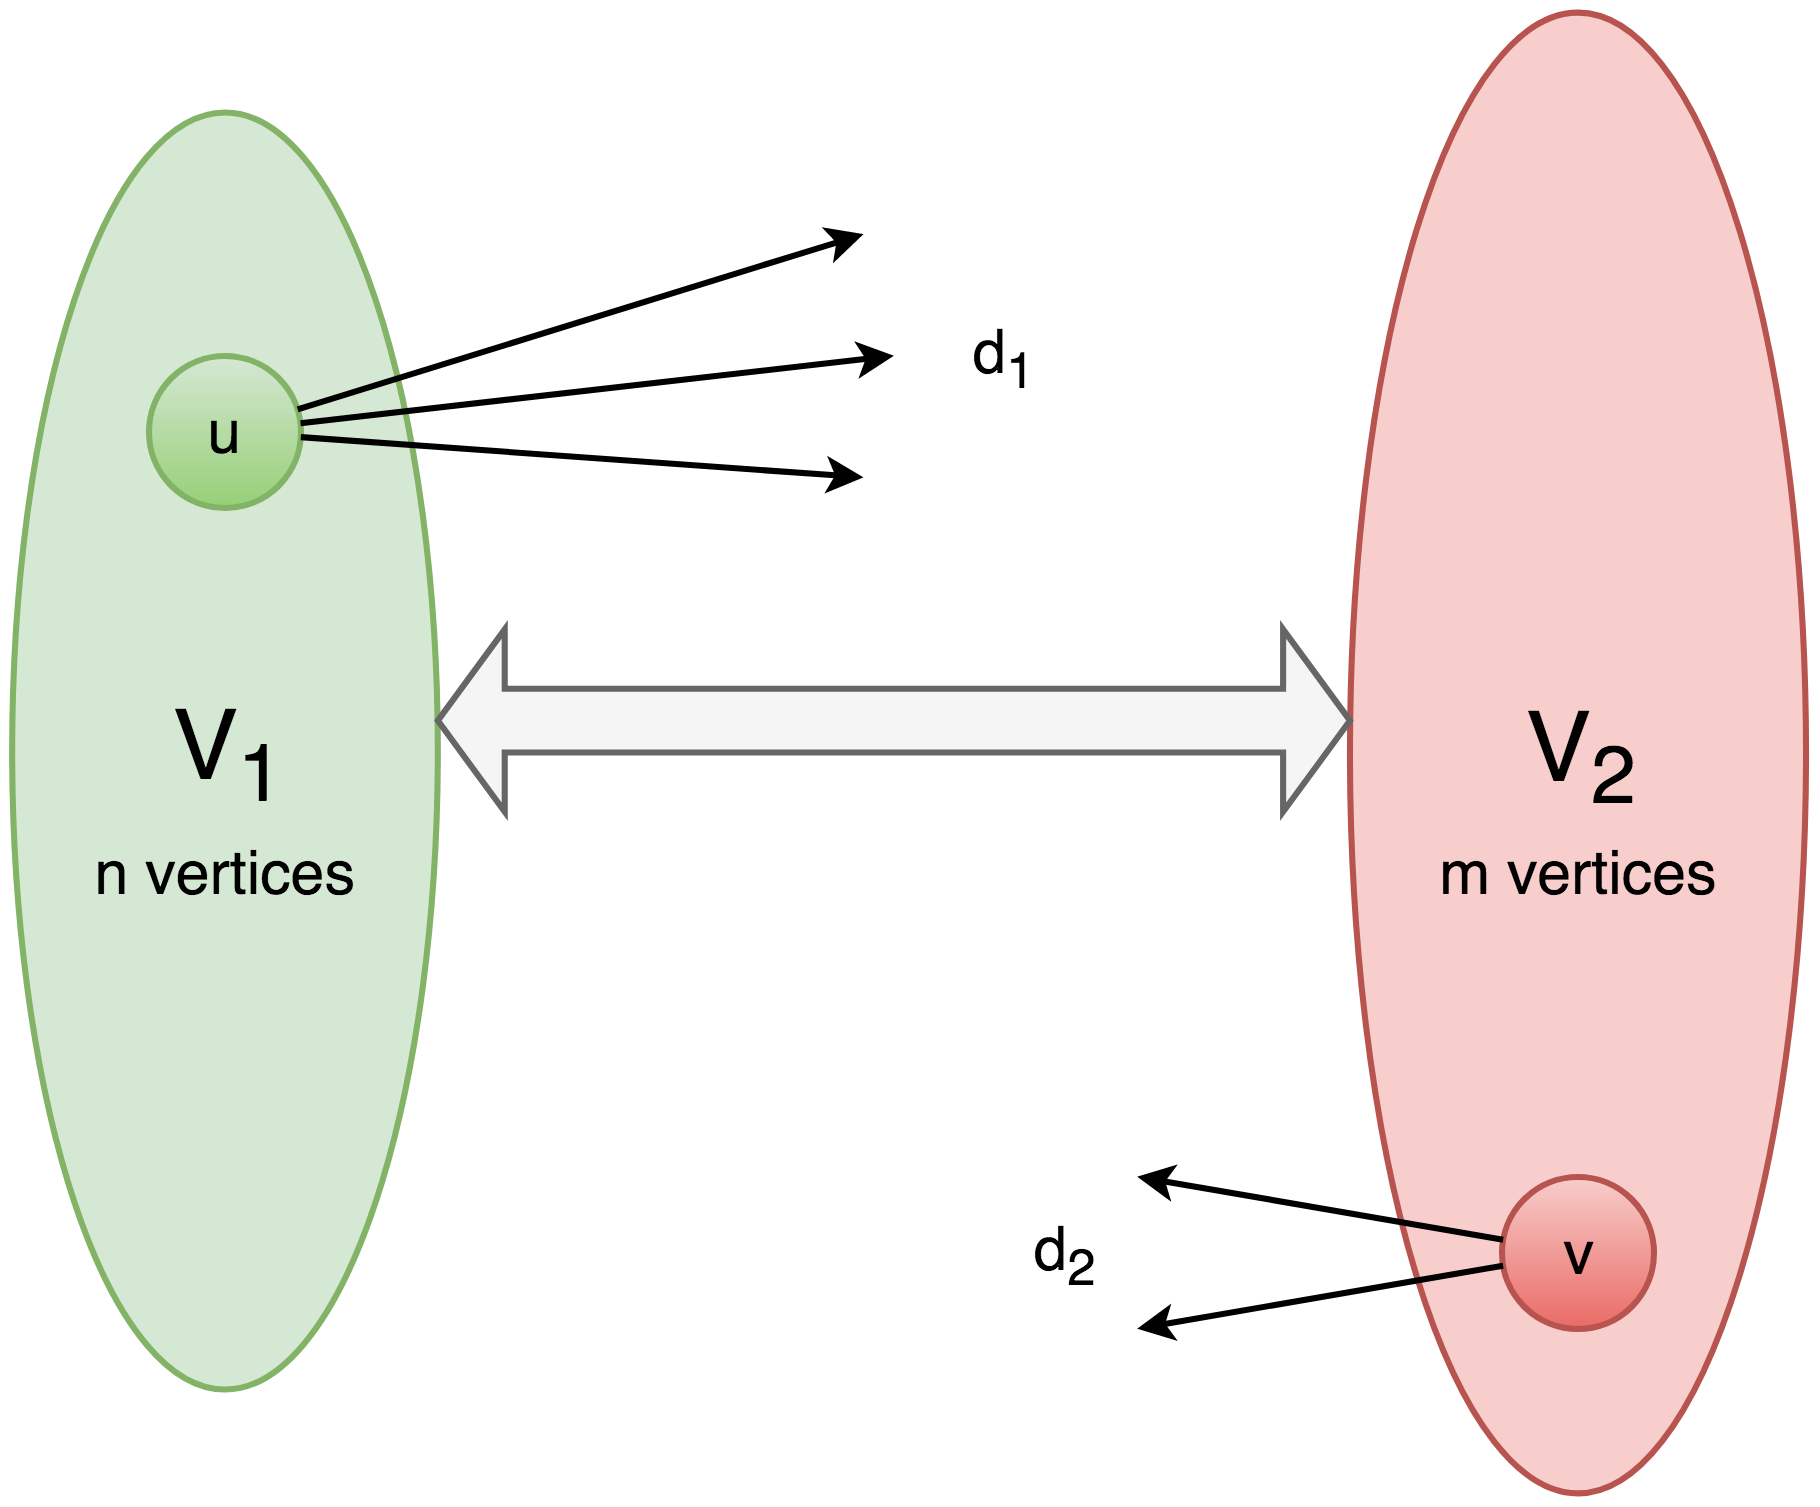
\includegraphics[width=0.5\linewidth]{bipartite_biregular_schematic.png}
\caption{The structure of a bipartite, biregular graph. 
	There are $n = |V_1|$ left vertices, $m=|V_2|$ right vertices,
    each of degree $d_1$ and $d_2$, with the constraint that
    $n d_1 = m d_2$.
	The distribution $\mathcal{G}(n,m,d_1,d_2)$ is taken uniformly over all such graphs.
    }
\label{fig:bipartite_schematic}
\end{figure}

Previous work on bipartite, biregular graphs
includes the work of \citet*{feng1996} and \citet*{li1996},
who proved the analog of the Alon-Boppana bound. 
For every $\epsilon >0$,
\begin{eqnarray}
\label{lower_bound}
\eta \geq \sqrt{d_1-1} + \sqrt{d_2 - 1} - \epsilon
\end{eqnarray}
as the number of vertices goes to infinity. 
This bound also follows immediately from the fact that 
the second largest eigenvalue cannot be asymptotically smaller 
than the right limit of the asymptotic 
support for the eigenvalue distribution,
which is $\sqrt{d_1-1} + \sqrt{d_2 - 1}$ and was first computed by
\citet*{godsil1988}.
They found the spectral measure 
$\mu(\lambda)$ has a point mass at $\lambda=0$ of size 
$\frac{1}{2} |d_1 - d_2| / (d_1 + d_2)$
and a continuous part given by the density

\begin{equation}
    \mathrm{d}\mu(\lambda) = 
    \frac{d_1 d_2 \sqrt{(- \lambda^2 + d_1 d_2 - (z - 1)^2)
                (\lambda^2 - d_1 d_2 + (z + 1)^2)}}
            {\pi (d_1 + d_2) (d_1 d_2 - \lambda^2) |\lambda|}~, 
    \label{eq:bipartite_esd}
\end{equation}
supported on 
$$|\sqrt{d_1-1} - \sqrt{d_2 - 1}| \leq |\lambda| \leq \sqrt{d_1-1} + \sqrt{d_2 - 1}~,~~\mbox{
where} ~~z=\sqrt{(d_1 - 1)(d_2 - 1)}~.$$
% As we will show here, this also follows from the Ihara-Bass formula
% \citep*{bass1992,kotani2000}, see section \ref{sec: connecting} \textcolor{red}{I don't have a proof of this from the Ihara-Bass formula}.

Graphs where $\eta$ attains the
Alon-Boppana bound, Eqn.~\eqref{lower_bound}, are also called Ramanujan.
Complete graphs are always Ramanujan but not sparse, 
whereas $d$-regular or bipartite $(d_1, d_2)$-regular graphs are sparse. 
Our results show that  
almost every $(d_1, d_2)$-regular graph is ``almost'' Ramanujan.

Beyond the first two eigenvalues, 
we should mention that \citet*{bordenave2010}
studied the limiting spectral distribution
of large sparse graphs.
They obtained a set of two coupled equations
that can be solved for the eigenvalue distribution of any
$(d_1, d_2)$-regular random graph. 
The solution of the coupled equations for fixed $d_1$ and $d_2$ shows convergence of the spectral distribution of a random regular bipartite graph to the Mar\v{c}enko-Pastur law. 
This was first observed by \citet*{godsil1988}. 
For $d_1, d_2 \to \infty$ with
$d_1/d_2$ converging to a constant, \citet*{dumitriu2016} showed that the limiting spectral distribution converges to a transformed version of the Mar\v{c}enko-Pastur law. When $d_1 = d_2 = d$, this is equal to the
Kesten-McKay distribution (\citet*{mckay1981}),
which becomes the 
semicircular law as $d \to \infty$
(\citet*{godsil1988, dumitriu2016}). 
Notably, \citet*{mizuno2003} 
obtained the same results when they calculated the asymptotic
distribution of eigenvalues for bipartite, biregular graphs of high girth.
However, their results are not applicable to 
random bipartite biregular graphs as these 
asymptotically almost surely have low girth (\citet*{dumitriu2016}).

Our techniques borrow heavily from the results of \citet*{bordenave2015a}
and \citet*{bordenave2015},
who simplified the trace method of \citet*{friedman2003a}
by counting non-backtracking walks built up of segments with at most one cycle, and by relating the eigenvalues of the adjacency matrix to the eigenvalues of the non-backtracking one via the Ihara-Bass identity.
The combinatorial methods we use to bound the number of 
such walks are similar to how 
\citet*{brito2015} counted self-avoiding walks
in the context of community recovery in a regular stochastic block model.


Finally, we should mention that similar techniques have been employed by \citet*{coste2017} 
to study the spectral gap of the Markov matrix of a random directed multigraph. 
The non-backtracking operator of a bipartite biregular graph 
could be seen as the adjacency matrix of a directed multigraph, 
whose eigenvalues are a simple scaling away from the eigenvalues of the Markov matrix of the same. 
However, the block structure of our non-backtracking matrix means that 
the corresponding multigraph is bipartite, 
and this makes it different from the model used in \citet*{coste2017}. 

\subsection{Configuration versus random lift model}\label{sec:1.2}

Random lifts are a model that allows the construction of large,
random graphs by repeatedly lifting the vertices of a base graph
and permuting the endpoints of copied edges.
See
\citet*{bordenave2015} for a recent overview.
A number of spectral gap results have been obtained for random lift models,
e.g.\ \citet*{friedman2003a,angel2007,friedman2014}, and \citet*{bordenave2015}.

Random lift models are contiguous with the configuration model 
in very particular cases.
See Section~\ref{sec:configuration_model} for a definition of 
the configuration model; 
this is a useful substitute for the uniform model and is practically 
equivalent.
For even $d$, 
random $n$-lifts of a single vertex with $d/2$ self-loops
are equivalent to the $d$-regular 
configuration model.
For odd $d$, no equivalent lift construction is known
or even believed to exist.

For $(d_1, d_2)$-biregular, bipartite
graphs the situation is more complicated.
A celebrated result due to \citet*{marcus2013} 
showed the existence of infinite
families of $(d_1, d_2)$-regular bipartite graphs that are Ramanujan.
That is, with 
$\eta = \sqrt{d_1-1} + \sqrt{d_2 - 1}$
by taking repeated lifts of the complete bipartite graph on $d_1$ left and $d_2$ right vertices $K_{d_1,d_2}$.
If $d_1=d_2=d$, then the configuration model is contiguous to 
the random lift of the multigraph with two vertices and
$d$ edges connecting then.
Certainly, for a biregular bipartite graph with
$n/d_2=m/d_1=k$ not an integer,
we cannot construct it by lifting $K_{d_1, d_2}$
as considered by \citet*{marcus2013}.
But even for $k$ integer, it seems likely the 
two models are not contiguous,
for the reasons we now explain.

Suppose there were a base graph $G$ that could be lifted to produce
any $(3,2)$-biregular, bipartite graph.
Consider another graph $H$ which is
a union of 2 complete bipartite graphs $K_{2,3}$.
Then $H$ is a $(3,2)$-biregular, bipartite graph and occurs
in the configuration model with nonzero probability. 
The only $G$ that $H$ could be a lift of is $K_{2,3}$, 
because it is a disconnected union and 
$K_{2,3}$ itself is not a lift of any graph or multigraph
(note that $2+3=5$ is prime). 
Therefore, $G$ would have to be $K_{2,3}$.
Figure~\ref{fig:disallowed_graph}
shows an example of another graph $H'$ with
the same number of vertices as $H$ which is $(3,2)$-biregular, 
bipartite but is {\em not} a lift of $K_{2,3}$.
Now, $H$ and $H'$ both occur in the configuration model with equal, 
nonzero probability.
Therefore, we cannot construct {\em every example} of a
$(3,2)$-biregular, bipartite graph
by repeatedly lifting a {\em single} base graph $G$. 
\begin{figure}[t!]
    \centering
    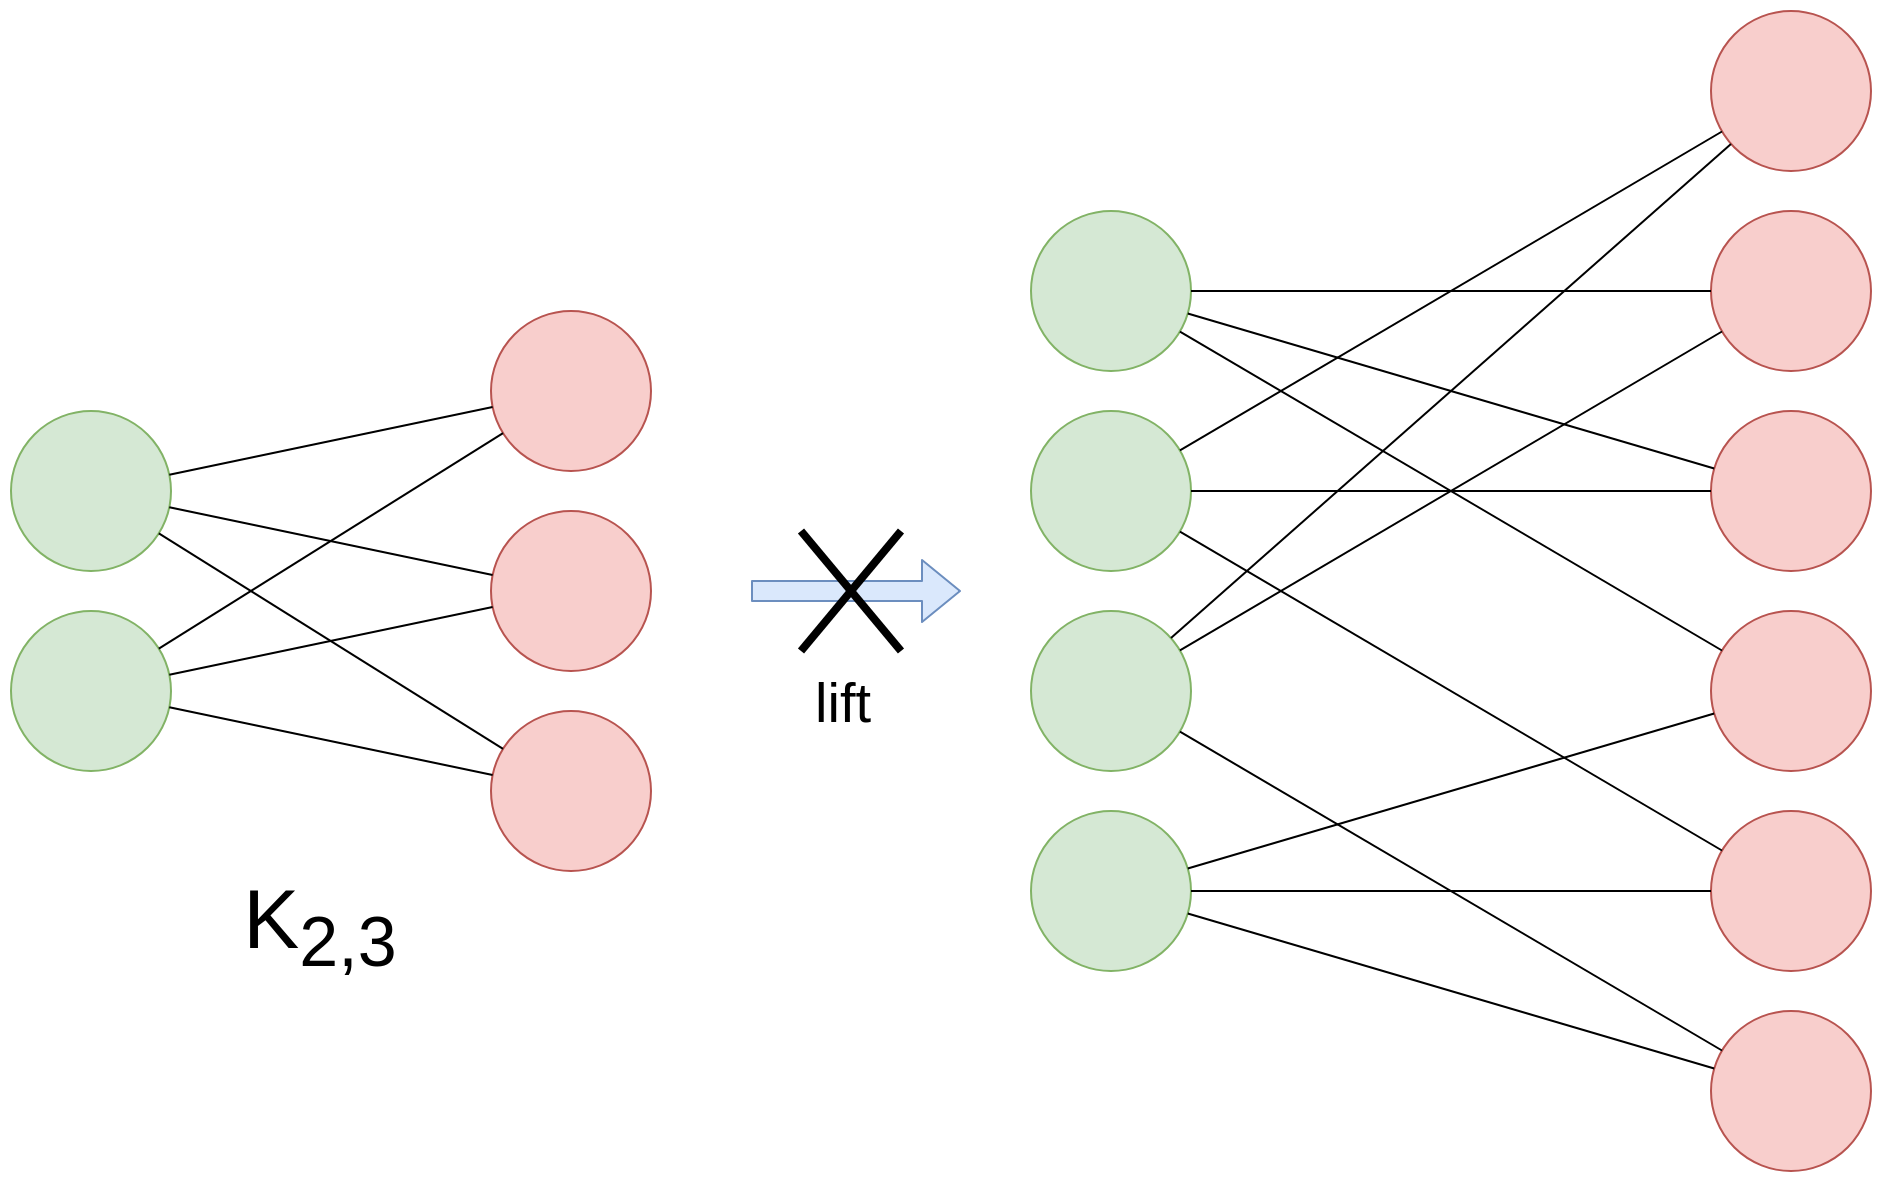
\includegraphics[width=0.5\linewidth]{Lift_counterexample_2.png}
    \caption{The $(3,2)$-bipartite, biregular 
        graph on the right is not a 2-lift of $K_{2,3}$.
        Every pair of left vertices shares a neighbor on the right.
    }
    \label{fig:disallowed_graph}
\end{figure}

Since the eventual goal of any argument based on lifts that also applies 
to the configuration model would have to show that almost all
bipartite, biregular graphs can be obtained by lifting and 
are sampled asymptotically uniformly from the lift model,
the above considerations suggest this argument would be 
highly non-trivial. 
We in fact doubt such an argument can be made.
Intuitively, in the configuration model edges occur
``nearly independently,'' 
whereas for random lifts there are strong dependencies 
due to the fact that many edges are not allowed;
see
\citet*{bordenave2015}.

\subsection{Structure of the paper}

Briefly, we now lay out the method of proof that the 
bipartite, biregular random graph is Ramanujan.
The proof outline is given in detail in Section~\ref{sec:proof_outline},
after some important preliminary terms and definitions given in 
Section~\ref{sec:preliminaries}.
The bulk of our work builds to Theorem~\ref{thm:gap_B},
which is actually a bound
on the second eigenvalue of the non-backtracking matrix $B$,
as explained in Section~\ref{sec:non_backtracking_matrix}.
The Ramanujan bound on the second eigenvalue of $A$ then follows 
as Theorem~\ref{cor:gap_A}.
As a side result, we find that row- and column-regular, rectangular 
matrices 
(the off-diagonal block $X$ of the adjacency matrix in Eqn.~\eqref{eq:matrix_blocks})
with aspect ratio smaller than one 
($d_1 \neq d_2$) have full rank with high probability.

To find the second eigenvalue of $B$,
we subtract from it a matrix $S$ that is formed from the leading eigenvectors,
and examine the spectral norm of the 
``almost-centered'' matrix $\bar{B} = B - S$.
We then proceed to use the trace method to bound 
the spectral norm of the matrix $\bar{B}^\ell$ by its trace.
However, since $\bar{B}$ is not positive definite, this leads us to consider
\[
\E\left(\|\bar{B}^{\ell}\|^{2k}\right)
\leq 
\E\left( \mathrm{Tr} \left( (\bar{B}^{\ell}) (\bar{B}^{\ell})^* \right)^{k} \right)~.
\]
On the right hand side, the terms in $\bar{B}^\ell$ refer to circuits built up of
$2k$ segments, each of length $\ell+1$,
since an entry $B_{ef}$ is a walk on two edges.
Because the degrees are bounded, it turns out that, for $\ell = O(\log (n))$,
the depth $\ell$ neighborhoods of every vertex contain at most one cycle---they are ``tangle-free.''
Thus, we can bound the trace by computing the expectation of the circuits that contribute,
along with an upper bound on their multiplicity, 
taking each segment to be $\ell$-tangle-free.

Finally, to demonstrate the usefulness of the spectral gap,
we highlight three applications of our bound.
In Section~\ref{sec:communities}, we show a community detection application. 
Finding communities in networks is important
for the areas of social network, bioinformatics,
neuroscience, among others.
Random graphs offer tractable models to study when detection and 
recovery are possible. 

We show here how our results lead to 
community detection in regular stochastic block models with 
arbitrary numbers of groups, using a very general theorem by
\citet*{wan2015}. 
Previously, \citet*{newman2014} studied the spectral density of such models,
and the community detection problem of the special case of 
two groups was previously studied by \citet*{brito2015} and \citet*{barucca2017}.

In Section~\ref{sec:codes}, 
we examine the application to linear
error correcting codes built from sparse expander graphs.
This concept was first introduced by \citet*{gallager1962}
who explicitly used random bipartite biregular graphs.
These ``low density parity check'' codes
enjoyed a renaissance in the 1990s, 
when people realized they were well-suited to modern computers.
For an overview, see \citet*{richardson2003,richardson2008}.
Our result yields an explicit lower bound on the minimum distance
of such codes, i.e.\ the number of errors that can be corrected.

The final application, in Section~\ref{sec:matrix_completion},
leads to generalized error bounds for matrix completion.
Matrix completion is the problem of reconstructing a matrix from
observations of a subset of entries.
\citet*{heiman2014} gave an algorithm for reconstruction of a
square matrix with low complexity as measured by
a norm $\gamma_2$, which is similar to the trace norm
(sum of the singular values,
also called the nuclear norm or Ky Fan $n$-norm).
The entries which are observed are at the nonzero entries 
of the adjacency matrix of a bipartite, biregular graph. 
The error of the reconstruction is bounded above by a factor which is proportional
to the ratio of the leading two eigenvalues, so that a graph with larger
spectral gap has a smaller generalization error.
We extend their results to rectangular graphs, 
along the way strengthening them by a constant factor of two. 
The main result of the paper gives an explicit bound in terms of $d_1$ and $d_2$.

As this paper was being prepared for submission, 
we became aware of the work of \citet*{deshpande2018}.
In their interesting paper, they use the {\it smallest} positive eigenvalue 
of a random bipartite lift to study convex relaxation techniques for random
not-all-equal-3SAT problems.
It seems that our main result addresses the
configuration model version of this constraint satisfaction problem,
the first open question listed at the end of \citet*{deshpande2018}.

\section{Non-backtracking matrix $B$}\label{sec2:B}

\label{sec:non_backtracking_matrix}

Given $G \sim \mathcal{G}(n,m,d_1,d_2)$, 
we define the non-backtracking operator $B$.
This operator is a linear endomorphism of $\R^{|\vec{E}|}$,
where $\vec{E}$ is the set of oriented edges of $G$ and $|\vec{E}| = 2|E|$.
Throughout this paper, we will use $V(H)$, $E(H)$, and $\vec{E}(H)$
to denote the vertices, edges, and oriented or directed edges
of a graph, subgraph, or path $H$.
For oriented edges $e=(u,v)$,
where $u$ and $v$ are the starting and ending vertices of $e$,
and $f=(s,t)$, define:
 \[
B_{ef}=
\begin{cases}
  1,&\textrm{if $v=s$ and $u\neq t$};\\
  0,& \textrm{otherwise}.
\end{cases}
\]
We order the elements of $\vec{E}$ as $\{e_1, e_2,\cdots,e_{2|E|}\}$, so that the first $|E|$ have end point in the set $V_2$. In this way, we can write
\[
B = 
\left(
\begin{array}{cc} 
0 & B^{(12)} \\
B^{(21)} & 0 
\end{array} 
\right) .
\]
for $|E| \times |E|$ matrices 
$B^{(12)}$ and $B^{(21)}$ with entries equal to $0$ or $1$.

We are interested in the spectrum of $B$. 
% Denote the spectrum of an operator $L$ by $\sigma(L)$. Set: 
% \[
% \sigma(B)=\{\lambda_1\geq \lambda_2\geq \cdots \geq \lambda_{2|E|}\}
% \]
Denote by $\onealpha$ the vector with first $|E|$ coordinates equal to $1$ and the last $|E|$ equal to $\alpha = \sqrt{d_1-1}/\sqrt{d_2-1}$. We can check that
\[
B \onealpha = B^* \onealpha =\lambda \onealpha
\]
for $\lambda=\sqrt{(d_1-1)(d_2-1)}$. 
By the Perron-Frobenius Theorem,
we conclude that $\lambda_1=\lambda$ 
and the associated eigenspace has dimension one. 
Also, one can check that if $\lambda$ is an eigenvalue of $B$ 
with eigenvector $v=(v_1,v_2)$, 
$v_i\in \mathbb{R}^{|E|}$ 
then $-\lambda$ is also an eigenvalue with eigenvector $v'=(-v_1,v_2)$. 
Thus, $\sigma(B)=-\sigma(B)$ and $\lambda_{2|E|}=-\lambda_1$. 

\subsection{Connecting the spectra of $A$ and $B$}\label{sec: connecting}

\begin{figure}[t]
\centering
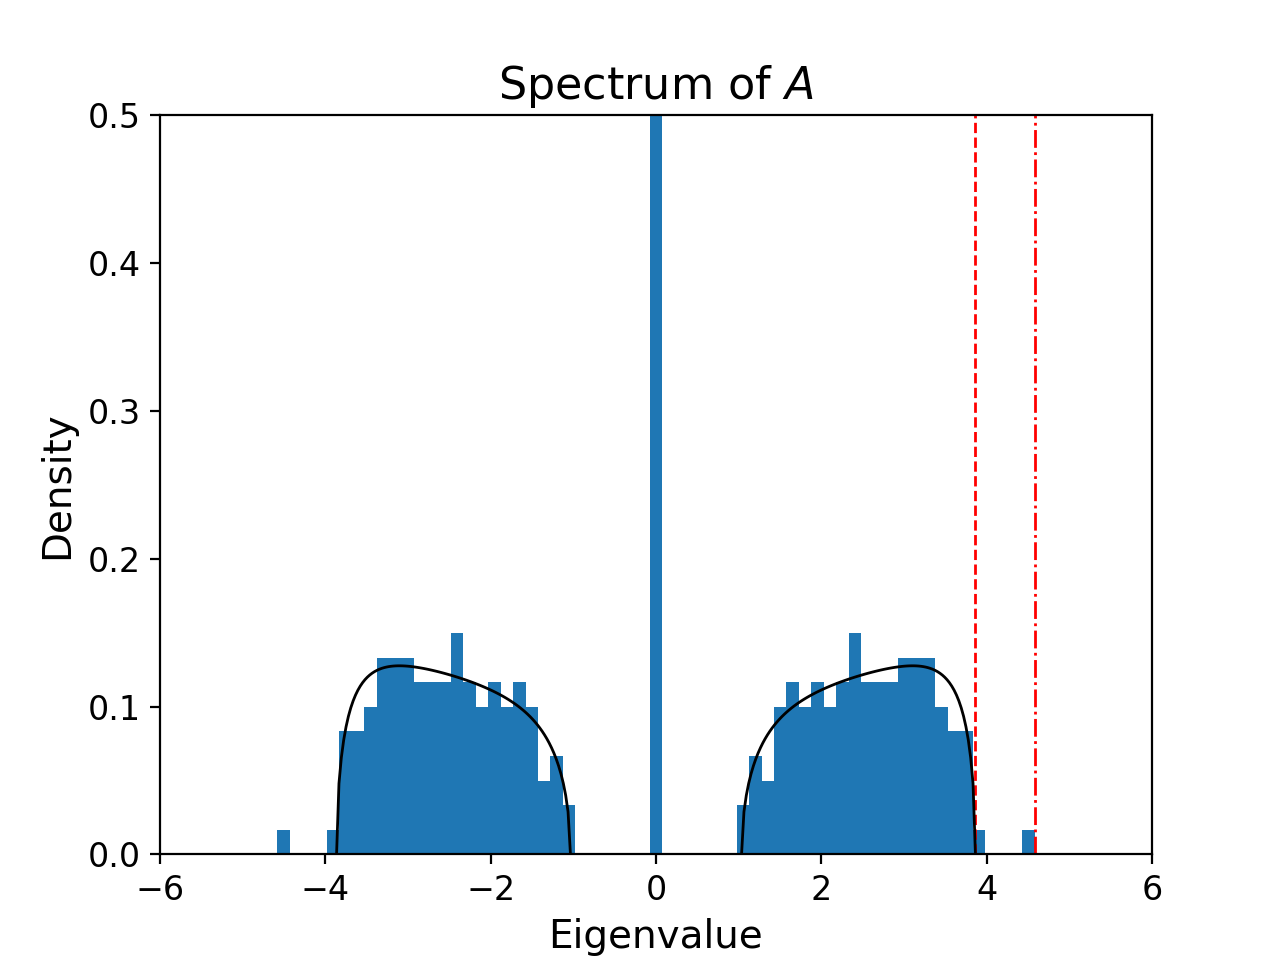
\includegraphics[trim={5 0 30 20},clip,width=0.49\linewidth]
{spectrum_n_400_k1_3_k2_7.png}
\hfill
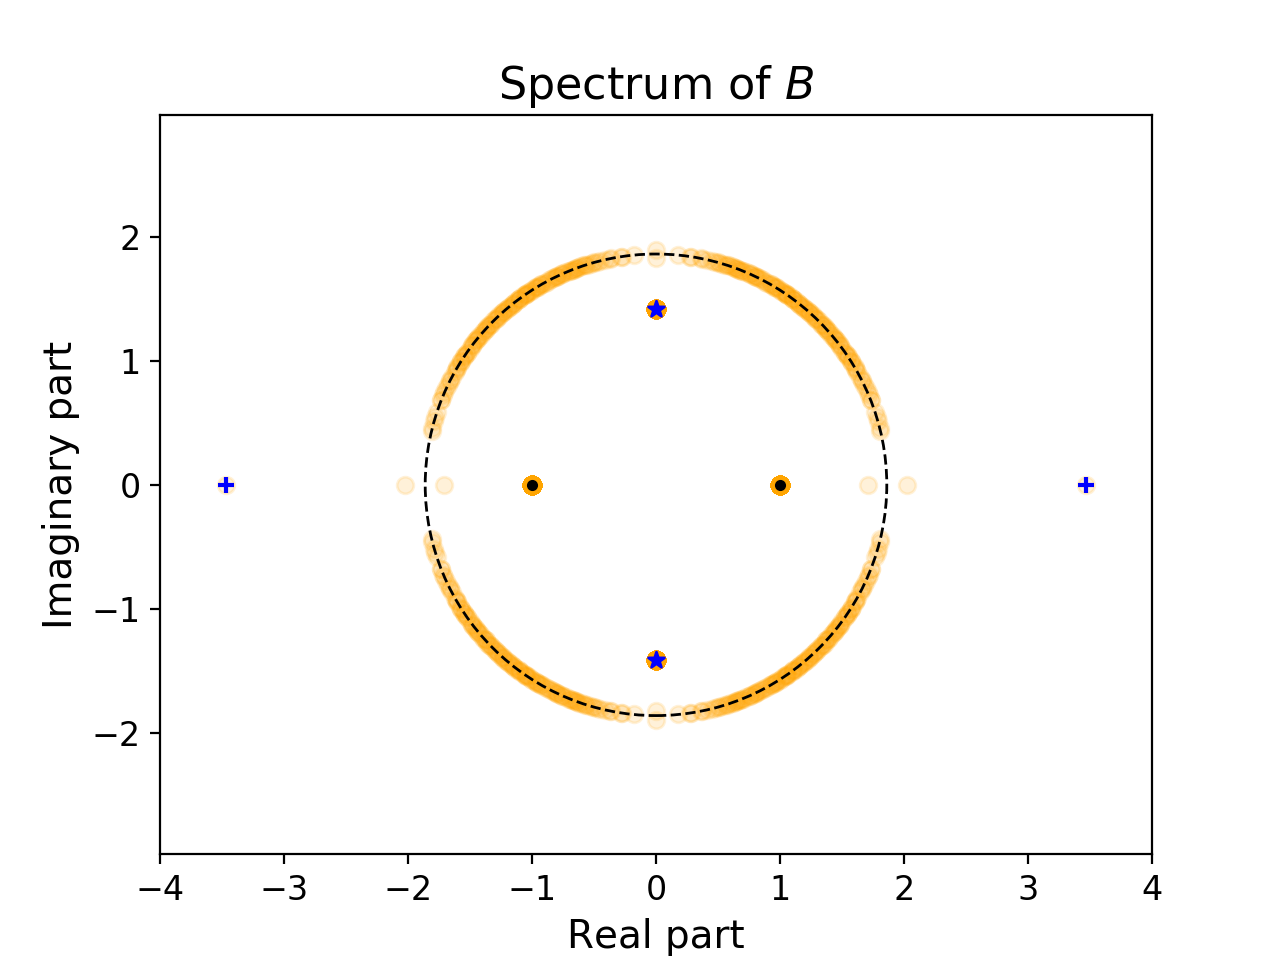
\includegraphics[trim={5 0 30 20},clip,width=0.49\linewidth]
{spectrum_B_n_400_k1_3_k2_7.png}
\caption{
Example spectra for a sample graph $G \sim \mathcal{G}(120, 280, 7, 3)$.
Left, we depict the spectrum of the adjacency matrix $A$.
The dash-dotted line marks the leading eigenvalue, while the 
dashed line marks our bound for the second eigenvalue, 
Theorem~\eqref{cor:gap_A}.
The Mar\u{c}enko-Pastur
limiting spectral density, Eqn.~\eqref{eq:bipartite_esd}, is shown in black.
Right, we depict the spectrum of the non-backtracking matrix
$B$ for the same graph. 
Each eigenvalue is shown as a transparent orange circle, 
the leading eigenvalues are marked with blue crosses, 
and the eigenvalues arising from zero eigenvalues of $A$ are marked with blue stars.
Our main result, Theorem~\ref{thm:gap_B}, 
proves that with high probability the non-leading eigenvalues
are inside, on, or very close to the black dashed circle.
In this case there are 8 outliers of the circle, which arise from 2 pairs of eigenvalues 
below and above the Mar\u{c}enko-Pastur bulk. 
}
\label{fig:spectrum_of_sample}
\end{figure}

Understanding the spectrum of $B$ turns out to be a challenging question. 
A useful result in this direction 
is the following theorem proved by \citet*{bass1992}, and subsequently in \citet*{watanabe2009} and \citet*{kotani2000};
see also Theorem 3.3 in \citet*{angel2015}.
\begin{theorem}[Ihara-Bass formula]\label{thm:ihara}
Let $G=(V,E)$ be any finite graph and $B$ be its non-backtracking matrix. 
Then
\[
\mathrm{det}(B-\lambda I) = (\lambda^2-1)^{|E|-|V|} 
  \mathrm{det}(D-\lambda A+\lambda^2 I),
\]
where $D$ is the diagonal matrix with $D_{vv}=d_v - 1$ 
and $A$ is the adjacency matrix of $G$. 
\end{theorem}
We use the Ihara-Bass formula to analyze the relationship of the spectrum of $B$ to the spectrum of $A$ in the case of a bipartite biregular graph.
It will turn out that this relationship can be completely unpacked. 
From Theorem~\ref{thm:ihara}, we get that
\[
\sigma(B)=\{\pm 1\}\bigcup\{\lambda:~ D-\lambda A+\lambda^2 I~\textrm{is not invertible}\}.
\]
Note that there are precisely $2(m+n)$ eigenvalues of $B$ that are determined by $A$, and that $\lambda = 0$ is not in the spectrum of $B$, since the graph has no isolated vertices ($\det(D) \neq 0$).

We use the special structure of $G$ to get a more precise description of $\sigma(B)$. 
The matrices $A$ and $D$ are equal to:
\[
A=\left(\begin{array}{cc} 0 & X \\
X^* & 0 \end{array}\right ),\ \
D=\left(\begin{array}{cc} (d_1-1)I_n & 0 \\
0 & (d_2-1)I_m \end{array}\right ),
\]
where $I_k$ is the $k\times k$ identity matrix.
Let $\lambda\in \sigma(B)\backslash\{-1,1\}$. 
Then there exists a nonzero vector $v$ such that
\[
(D-\lambda A+\lambda^2 I)v = 0 .
\]
Writing $v=(v_1,v_2)$ with $v_1\in \mathbb{C}^n$, $v_2\in \mathbb{C}^m$, we obtain:
\begin{eqnarray} 
\label{eq:sv_1}
Xv_2 & =& \frac{d_1-1+\lambda^2}{\lambda}v_1, \\
\label{eq:sv_2} 
X^*v_1 & = &\frac{d_2-1+\lambda^2}{\lambda}v_2~.
\end{eqnarray}    
The above imply that, provided that the right hand side is non-zero, 
\begin{eqnarray} 
\label{eq:quadratic_1}
\xi^2=\frac{(d_1-1+\lambda^2)(d_2-1+\lambda^2)}{\lambda^2}
\end{eqnarray}
is a nonzero eigenvalue of both $XX^*$ with eigenvector $v_1$ and $X^*X$, with eigenvector $v_2$.
We can rewrite Eqn.~\eqref{eq:quadratic_1} as
\begin{eqnarray} 
\label{eq:quadratic_2}
\lambda^4 - (\xi^2 - d_1 - d_2+2) \lambda^2 + (d_1-1)(d_2-1) = 0~.
\end{eqnarray}

%From this relation we can derive the lower bound in \eqref{lower_bound} as follows, for any $\epsilon>0$, if $|\lambda_2|<\sqrt{d_1-1}+\sqrt{d_2-1}-\epsilon$ we get $|\eta^2-d_1-d_2-2|< 2\sqrt{(d_1-1)(d_2-1)}$

We will now detail how the eigenvalues of $A$ (denoted $\xi$ here) 
map to eigenvalues of $B$ and vice-versa.
Let us examine the special case $\xi = 0$. Assume $n \leq m$ for simplicity.
Assume that the rank of $X$ is $r$. 
Then $X$ has $m-r$ independent vectors in its nullspace. 
Let $u$ be one such vector. 
Now, if we pick $v_2 = u$, $v_1 = 0$, and $\lambda = \pm i \sqrt{d_2-1}$,
Eqns.~\eqref{eq:sv_1} and \eqref{eq:sv_2} are satisfied. 
Hence, $\pm i \sqrt{d_2-1}$ are eigenvalues of $B$, both with multiplicity $m-r$. 

Since the rank of $X$ is $r$, it follows that the nullity of $X^*$ is $n-r$, 
so there are $n-r$ independent vectors $w$ for which $X^*w = 0$. 
Now, note that picking $v_1 = w$, $v_2 = 0$, and $\lambda = \pm i \sqrt{d_1 -1}$, 
we satisfy Eqns.~\eqref{eq:sv_1} and \eqref{eq:sv_2}. 
Thus, $\pm i \sqrt{d_1-1}$ are eigenvalues of $B$, both with multiplicity $n-r$.

The remaining $4r$ eigenvalues of $B$ determined by $A$ come from nonzero
eigenvalues of $A$.
For each $\xi^2$ with $\xi$ a nonzero eigenvalue of $A$, 
we will have precisely $4$ complex solutions to Eqn.~\eqref{eq:quadratic_1}. 
Since there are $2r$ such eigenvalues, 
coming in pairs $\pm \xi$, they determine a total of $4r$ eigenvalues of $B$, 
and the count is complete.  
To summarize the discussion above, we have the following Lemma:
\begin{lemma} 
\label{A2B} 
Any eigenvalue of $B$ belongs to one of the following categories:
\begin{enumerate}
\item $\pm 1$ are both eigenvalues with multiplicities $|E|-|V| = nd_1 - m -n$,
\item $\pm i \sqrt{d_1-1}$ are eigenvalues with multiplicities $m-r$, where $r$ is the rank of the matrix $X$,
\item $\pm i \sqrt{d_2-1}$ are eigenvalues with multiplicities $r$, and
\item every pair of non-zero eigenvalues $(-\xi, \xi)$ of $A$ generates exactly $4$ eigenvalues of $B$. 
\end{enumerate}
\end{lemma}

\section{Main result}

We spend the bulk of this paper in the proof of the following:
\begin{theorem}
\label{thm:gap_B} 
If $B$ is the non-backtracking matrix of a bipartite, biregular random graph
$G \sim \mathcal{G}(n,m,d_1,d_2)$,
then its second largest eigenvalue
\[
|\lambda_2 (B)| \leq ((d_1-1)(d_2-1))^{1/4}+\epsilon_n
\]
asymptotically almost surely, with $\epsilon_n \to 0$ as $n \to \infty$. Equivalently, there exists a sequence $\epsilon_n \rightarrow 0$ as $n \rightarrow \infty$ so that 
\[
\mathbb{P}\left [ |\lambda_2(B)| - ((d_1-1)(d_2-1))^{1/4} >\epsilon_n \right ] \rightarrow 0 ~~\mbox{as}~~ n \rightarrow \infty~.
\]
\end{theorem}
% * <dumitriu@uw.edu> 2017-11-29T18:49:27.533Z:
%
% ^.
\begin{remark}
For the random lift model, Theorem \ref{thm:gap_B} was proved by \citet*{bordenave2015}, which applies to random bipartite graphs only when $d_1=d_2=d$ as discussed in section \ref{sec:1.2}. 
\end{remark}
We combine Theorems \ref{thm:ihara} and \ref{thm:gap_B} to prove our main result concerning the spectrum of $A$.   
\begin{theorem}[Spectral gap]
\label{cor:gap_A}
Let
$
A=\left(\begin{array}{cc} 0 & X \\
X^* & 0 \end{array}\right )
$
be the adjacency matrix of a bipartite, biregular random graph
$G \sim \mathcal{G}(n,m,d_1,d_2)$. 
Without loss of generality, assume $d_1 \geq d_2$ or, equivalently, $n \leq m$.
Then:
\begin{enumerate}[(i)]
\item Its second largest eigenvalue $\eta = \lambda_2 (A)$ satisfies
%\label{gap}
\[
\eta \leq \sqrt{d_1-1}+\sqrt{d_2-1}+ \epsilon_n'
\]
asymptotically almost surely, with $\epsilon_n' \to 0$ as $n \to \infty$.
\item  Its smallest positive eigenvalue $\eta^+_{\rm min} = \min ( \{\lambda \in \sigma(A): \lambda > 0\} )$ satisfies
\[
\eta_{\rm min}^+\geq \sqrt{d_1-1}-\sqrt{d_2-1}- \epsilon_n''
\]
asymptotically almost surely, with $\epsilon_n''\to 0$ as $n \to \infty$. (Note that this will be almost surely positive if $d_1>d_2$; no further information is gained if $d_1 = d_2$.)
\item If $d_1 \neq d_2$, the rank of $X$ is $n$ with high probability.
\end{enumerate}
\end{theorem}

\begin{remark}
Since the first draft of this work came out, considerable advances haven been made regarding the question of singularity of random regular graphs. It was conjectured in \citet*{costello2008} that, for $3\leq d\leq n-3$, the adjacency matrix of uniform $d$-regular graphs is not singular with high probability as $n$ grows to infinity. For directed $d$-regular graphs and growing $d$, this is now known to be true, following the results of \citet*{cook2017} and \citet*{litvak2016, litvak2017}. 
For constant degree $d$, \citet*{huang2018a,huang2018b} proved the asymptotic non-singularity of the adjacency matrix for both undirected and directed $d-$regular graphs. The last case can be interpreted as singularity of the adjacency matrix of random $d-$regular bipartite graph. To the best of our knowledge, Theorem~\ref{cor:gap_A}(iii) is the first result concerning the rank of rectangular random matrices with $d_1$ nonzero entries in each row and $d_2$ in each column.  
%The problem of investigating the rank of adjacency matrices of  random regular graphs is quite challenging. It was conjectured in \citet*{costello2008} that, for $3\leq d\leq n-3$, the adjacency matrix of uniform $d$-regular graphs is not singular with high probability as $n$ grows to infinity. For directed $d$-regular graphs and growing $d$, this is now known to be true, following the results of \citet*{cook2017} and \citet*{litvak2016, litvak2017}. For constant $d$, \citet*{litvak2018} proved that the rank is at least $n-1$ with high probability as $n$ grows to infinity. To the best of our knowledge, Theorem~\ref{cor:gap_A}(iii) is the first result concerning the rank of rectangular random matrices with $d_1$ nonzero entries in each row and $d_2$ in each column.  
\end{remark}

\begin{remark} The analysis of the Ihara-Bass formula for Markov matrices of bipartite biregular graph appeared before in \citet*{kempton2016}. We have independently proven Lemma~\ref{A2B} and extracted from it more information than is given in \citet*{kempton2016}, including Theorem~\ref{cor:gap_A}(iii). 
\end{remark}

\begin{proof}
Eqn.~\eqref{eq:quadratic_2}, describing those eigenvalues of $B$ which are neither $\pm 1$ and do not correspond to $0$ eigenvalues of $A$, is equivalent to
\begin{eqnarray} 
\label{eq:quadratic_in_xy}
0 = x^2 + \alpha \beta - (y - \alpha - \beta ) x,
\end{eqnarray}
where $x = \lambda^2$, $y = \xi^2$, $\alpha = d_1 - 1$, and $\beta = d_2 -1$. 
% Solving for $y$, we find that
% \[
% y = f(x) = x + \frac{\alpha \beta}{x} + \alpha + \beta .
% \]
% It is a simple exercise to see that in order to have $y$ real, we need to have either that $x$ is real, or that $x$ is on the circle of radius $\sqrt{\alpha \beta}$. 
A simple discriminant calculation and analysis of 
Eqn.~\eqref{eq:quadratic_in_xy}, keeping in mind that $y \neq 0$,  
leads to a number of cases in terms of $y$:
\begin{enumerate}[{Case} 1:]
%\item $y = 0$ leads to solutions $x_{+} = -\beta$ and $x_{-} = -\alpha$,
%meaning the eigenvalues $\lambda$ are $i \sqrt{\beta}$ and $i \sqrt{\alpha}$. 
\item $y \in ((\sqrt{\alpha} -\sqrt{\beta})^2, (\sqrt{\alpha} + \sqrt{\beta})^2)$,
i.e.\ roughly speaking, $\eta$ is in the bulk,
means that $x$ is on the circle of radius $\sqrt{\alpha \beta}$ and the
corresponding pair of eigenvalues $\lambda$ are on a circle of radius 
$(\alpha \beta)^{1/4}$.

\item $y \in (0, (\sqrt{\alpha} - \sqrt{\beta})^2]$ means that $x$ is real and negative, so $\lambda$ is purely imaginary.
%\item $|\lambda_2| \leq ((d_1-1)(d_2-1))^{1/4} + \epsilon$ 
%with high probability implies that if 
%$d_1 \neq d_2$, 
%$r=n$ with high probability.
%Otherwise, we would have eigenvalues of $B$ with 
%absolute value $\sqrt{d_1-1}$ 
%and this is larger than $((d_1-1)(d_2-1))^{1/4}$.

In this case, one may also show that the smaller of the two possible values 
for $x$ is increasing as a function of $y$ and
$x_{-} \in (-\alpha, -\sqrt{\alpha \beta}]$. 
The larger of the two values of $x$ is decreasing and $x_{+} \in [-\sqrt{\alpha \beta}, - \beta)$.
Correspondingly, the largest in absolute value that 
$\lambda$ could be in this case 
is $\pm i \alpha^{1/4} = \pm i (d_1-1)^{1/4}$. 

\item $y \geq (\sqrt{\alpha} + \sqrt{\beta})^2$ means that 
both solutions $x_{\pm}$ are real,
and the larger of the two is larger than $\sqrt{\alpha \beta}$.
\end{enumerate}

Note that Eqn.~\ref{eq:quadratic_in_xy} 
shows there is a continuous dependence between $x$ and $y$, 
and consequently between $\xi$ and $\lambda$.
Putting these cases together with Lemma \ref{A2B}, a few things become apparent:
\begin{enumerate}
\item $\xi>\sqrt{d_1-1}+ \sqrt{d_2-1}$ means that 
$\lambda> ((d_1-1)(d_2-1))^{1/4}$.
\item $|\lambda_2| \leq ((d_1-1)(d_2-1))^{1/4} + \epsilon$ 
implies that all eigenvalues except for the largest two 
will be either $0$, or in a small neighborhood 
$[\sqrt{\alpha} -\sqrt{\beta} - \delta, 
\sqrt{\alpha} + \sqrt{\beta} + \delta]$ 
of the bulk, with $\delta$ small if $\epsilon$ is small since the dependence of $\delta$ on $\epsilon$ can be deduced from Eqn.~\ref{eq:quadratic_in_xy}. 
\item $|\lambda_2| \leq ((d_1-1)(d_2-1))^{1/4} + \epsilon$ 
with high probability implies that if 
$d_1 \neq d_2$, 
$r=n$ with high probability.
Otherwise, we would have eigenvalues of $B$ with 
absolute value $\sqrt{d_1-1}$ 
and this is larger than $((d_1-1)(d_2-1))^{1/4}$.
\end{enumerate}
This completes the proof, with results (i) and (ii) following from the point 2 and (iii) following from point 3.
\end{proof}


In Fig.~\ref{fig:spectrum_of_sample}, 
we depict the spectra of $A$ and $B$ for a sample graph
$G \sim \mathcal{G}(120,280,7,3)$.
Looking at the non-backtracking spectrum, 
we observe the two leading eigenvalues $\pm \sqrt{(d_1 - 1 )(d_2 - 1)}$
(blue crosses) outside the circle of radius 
$((d_1 - 1)(d_2 - 1))^{1/4}$
along with a number of zero eigenvalues (black dots).
There are also multiple purely imaginary eigenvalues 
which can arise from $|\xi| \in (0, \sqrt{d_1 - 1} - \sqrt{d_2 - 1}]$
as well as $\xi = 0$.
However, due to Theorem~\ref{cor:gap_A},
only the smaller of $i \sqrt{d_1 - 1}$ and $i \sqrt{d_2 - 1}$ 
is observed with non-negligible probability,
implying that $X$ has rank $r = n$ with high probability
(shown as blue stars).
Furthermore, we observe two pairs of real eigenvalues of $B$ which are connected to a pair of eigenvalues of $A$ from ``above'' the bulk, as well as two pairs of imaginary eigenvalues of $B$ which are connected to a pair of eigenvalues of $A$ from ``below'' the bulk.
